\documentclass{beamer}
\usepackage[utf8]{inputenc}
\usepackage[T1]{fontenc}
\usepackage[frenchb]{babel}

\usetheme{Madrid}
\usecolortheme{whale}
\beamertemplatenavigationsymbolsempty

\title{\textbf{Recalage et fusion de modèles numérisés\\tridimensionnels de grande taille}}
\subtitle{MEMO-F-403 - Préparation au mémoire}
\author{Tim Lenertz}
\date{2 septembre 2014}
\institute{ULB}

\maketitle

\begin{document}

\begin{frame}
\frametitle{Introduction}
	\begin{columns}
	\begin{column}[T]{.7\textwidth}
		\begin{itemize}
		\item \textbf{Nuage de points}\\
			= ensemble de points sur surface d'objet
		\item Pas de connectivité des points
		\item Pris par scanner laser, photogrammétrie
		\item Coordonnées dans repère cartésien 3D 
		\item Attribués par couleur RGB, température, etc.
		\item Documentation 3D \\
			(site archéologiqes, bâtiment, grotte, terrain, dent, objet céleste, ...)
		\end{itemize}
	\end{column}
	\begin{column}[T]{.3\textwidth}
		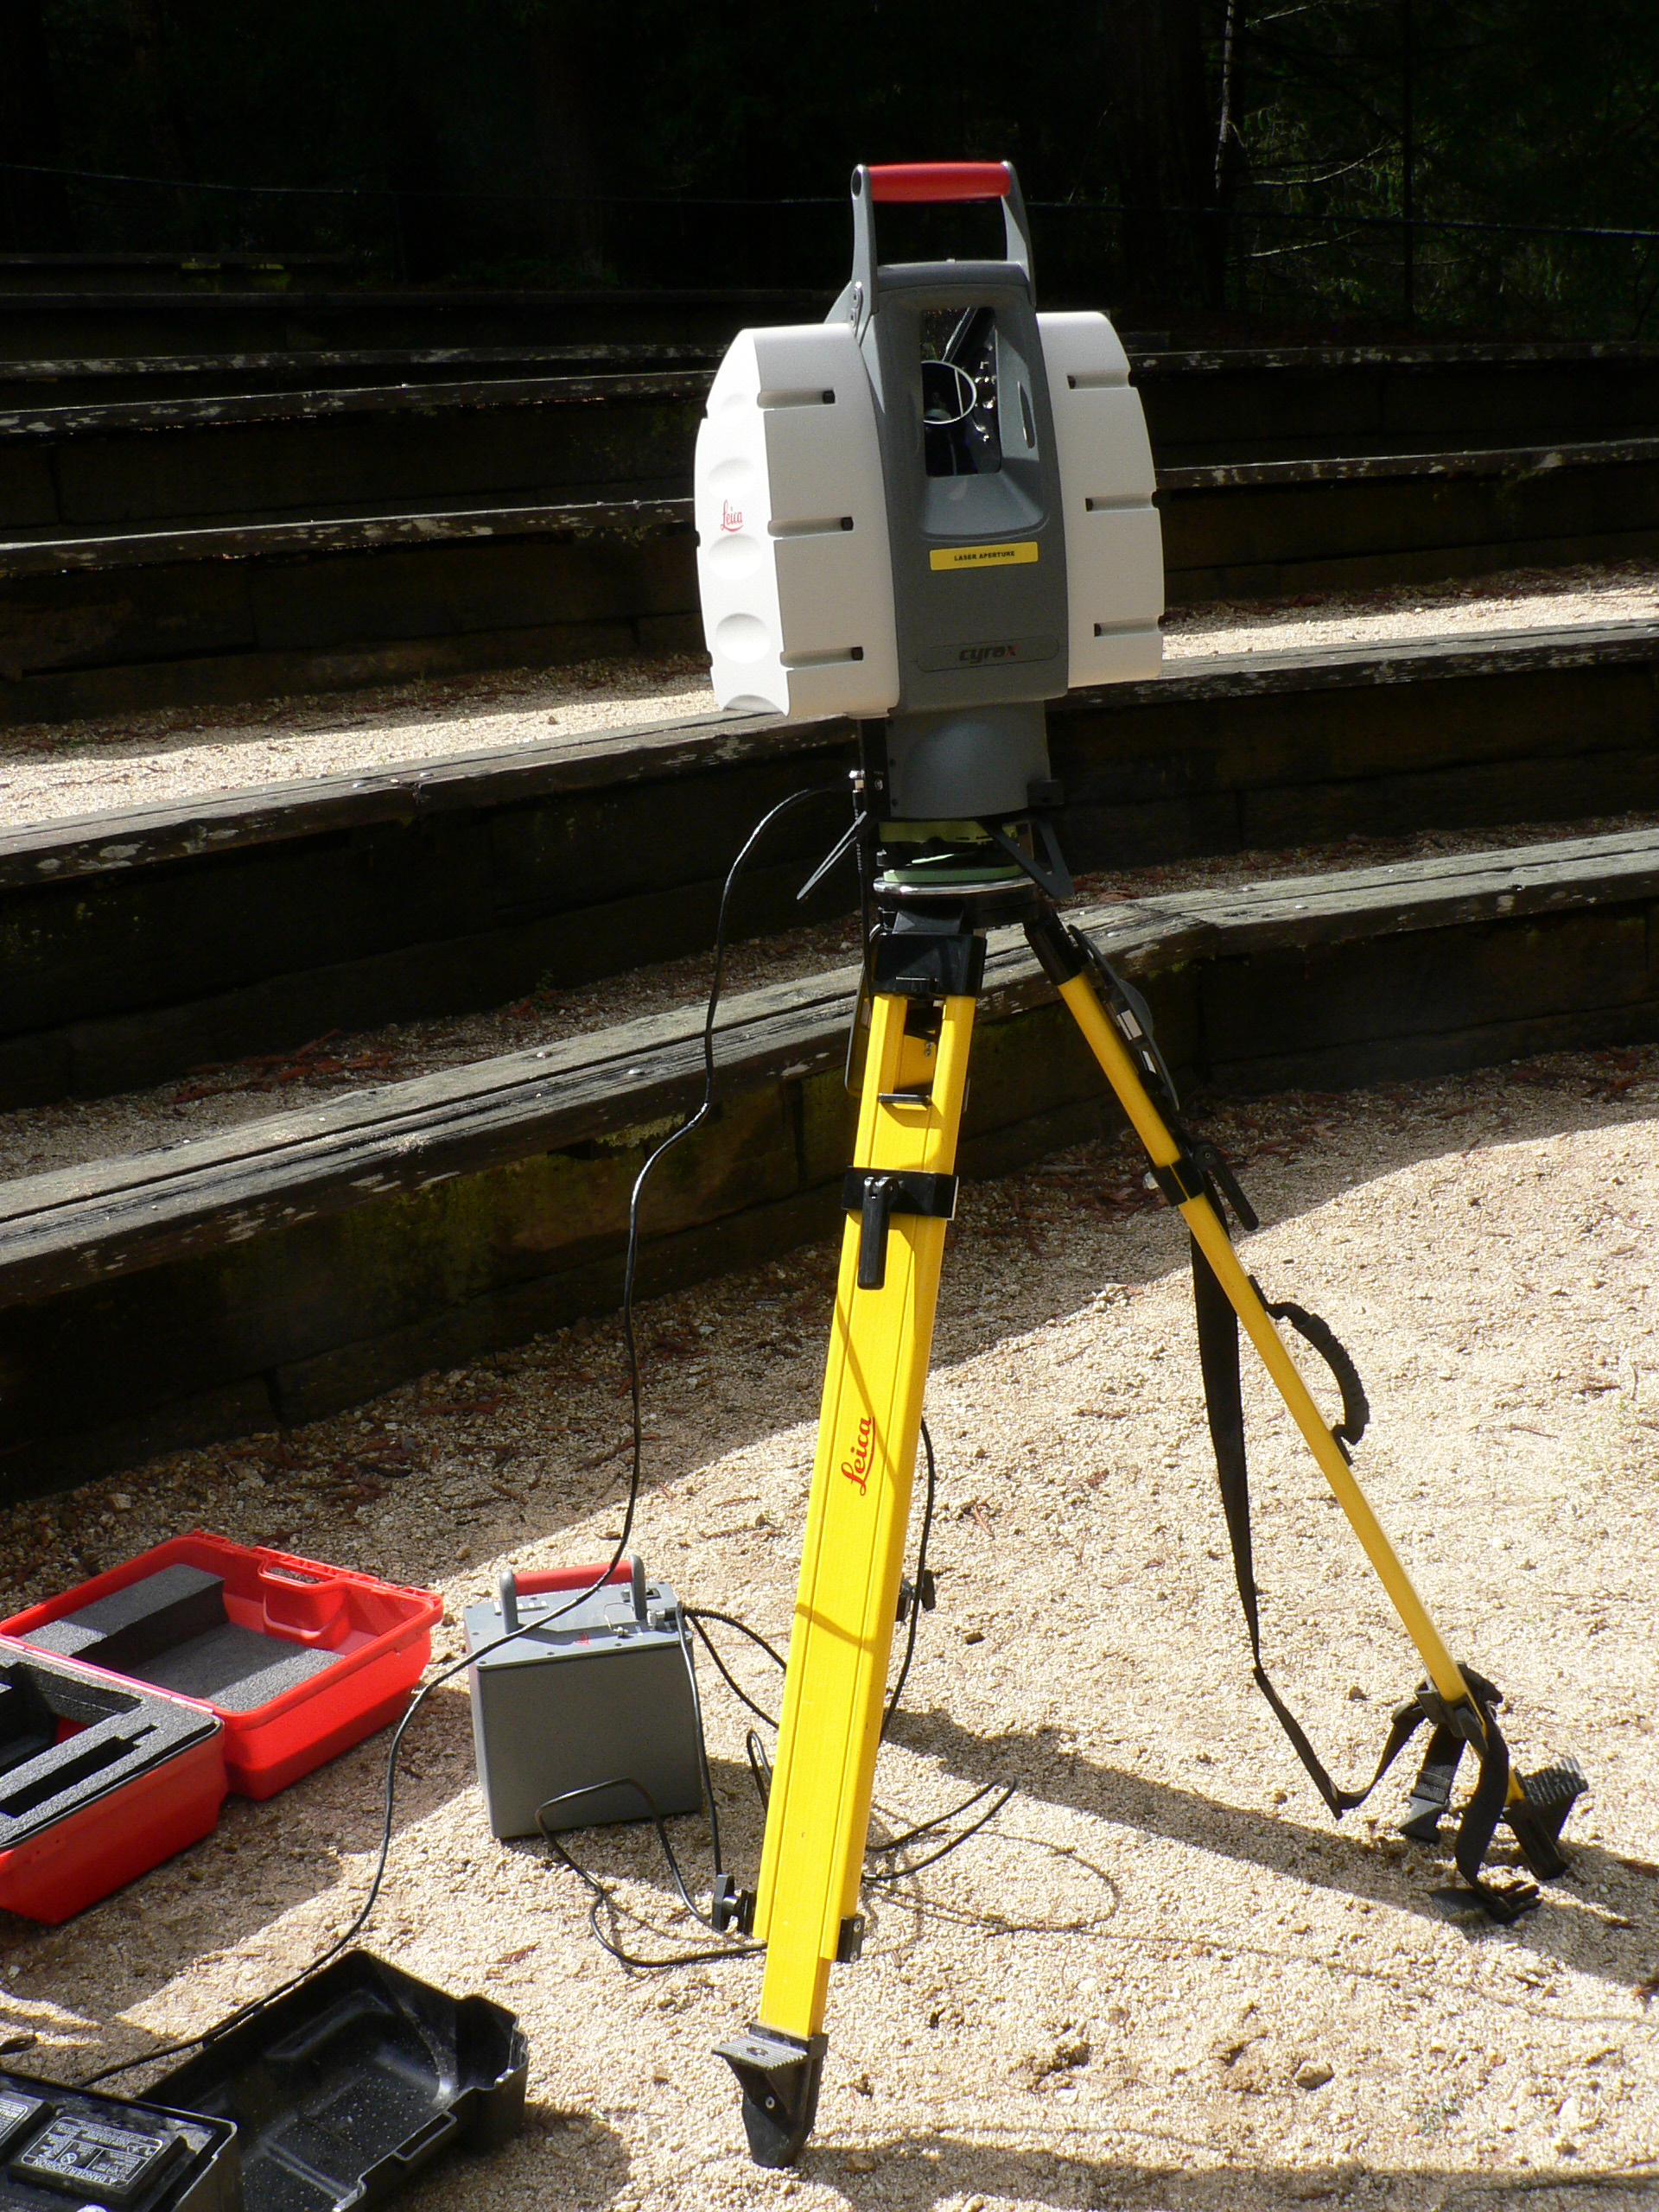
\includegraphics[width=\textwidth]{lidar.jpg}
		\\ \footnotesize Scanner LIDAR
	\end{column}
	\end{columns}
\end{frame}

\begin{frame}
\frametitle{Nuage de points - Exemple 1}
	\center
	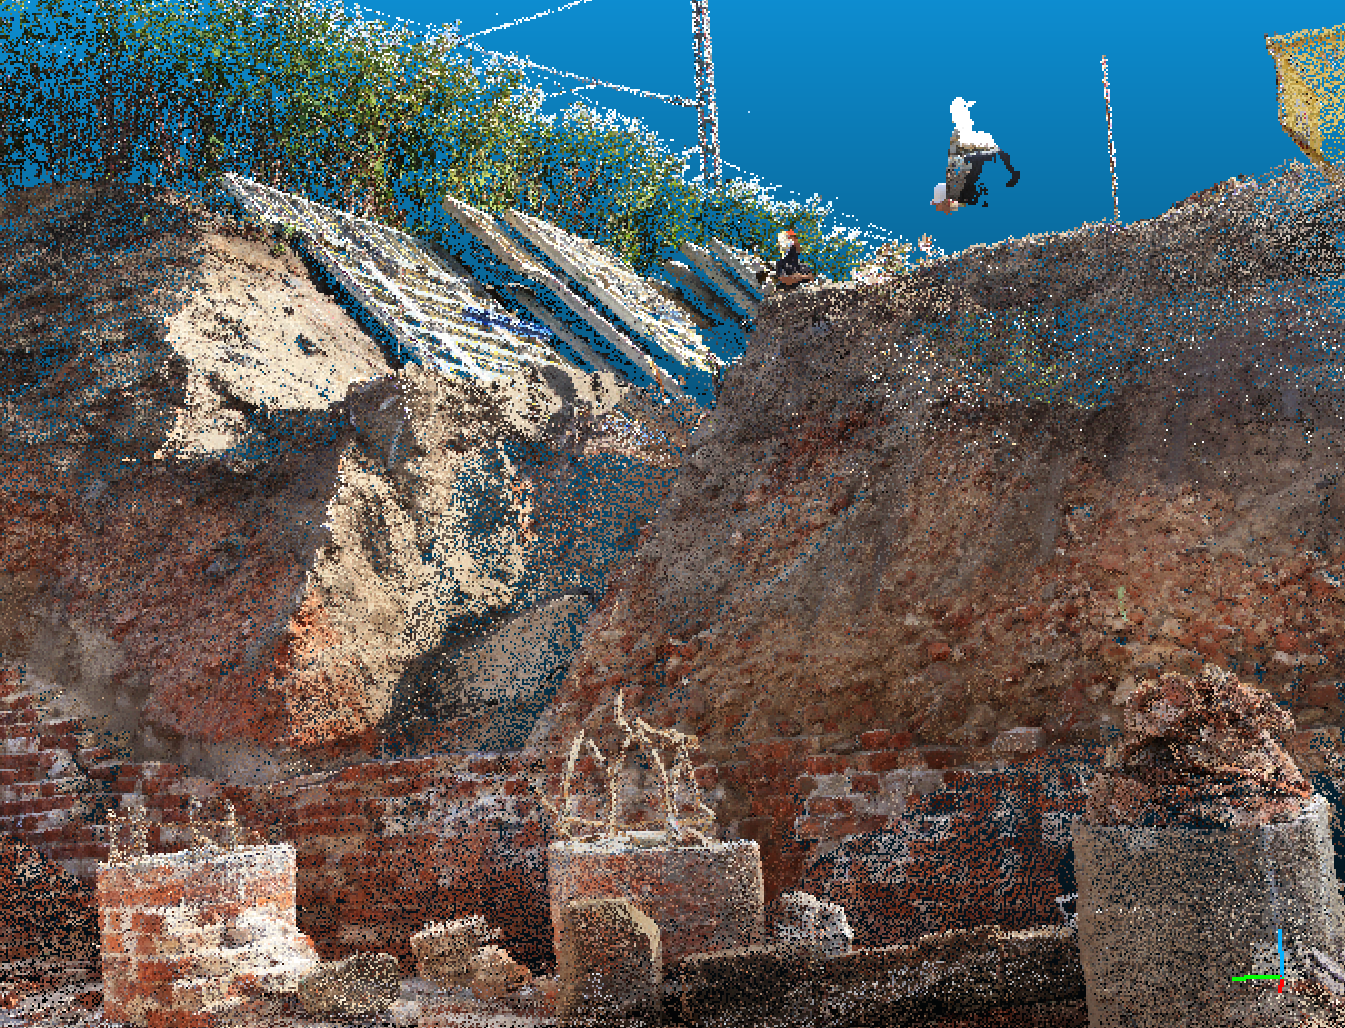
\includegraphics[width=.8\textwidth]{tower_screenshot.png} \\
	\footnotesize{Modèle de Jacobs University Bremen gGmbH}
\end{frame}

\begin{frame}
\frametitle{Nuage de points - Exemple 2}
	\center
	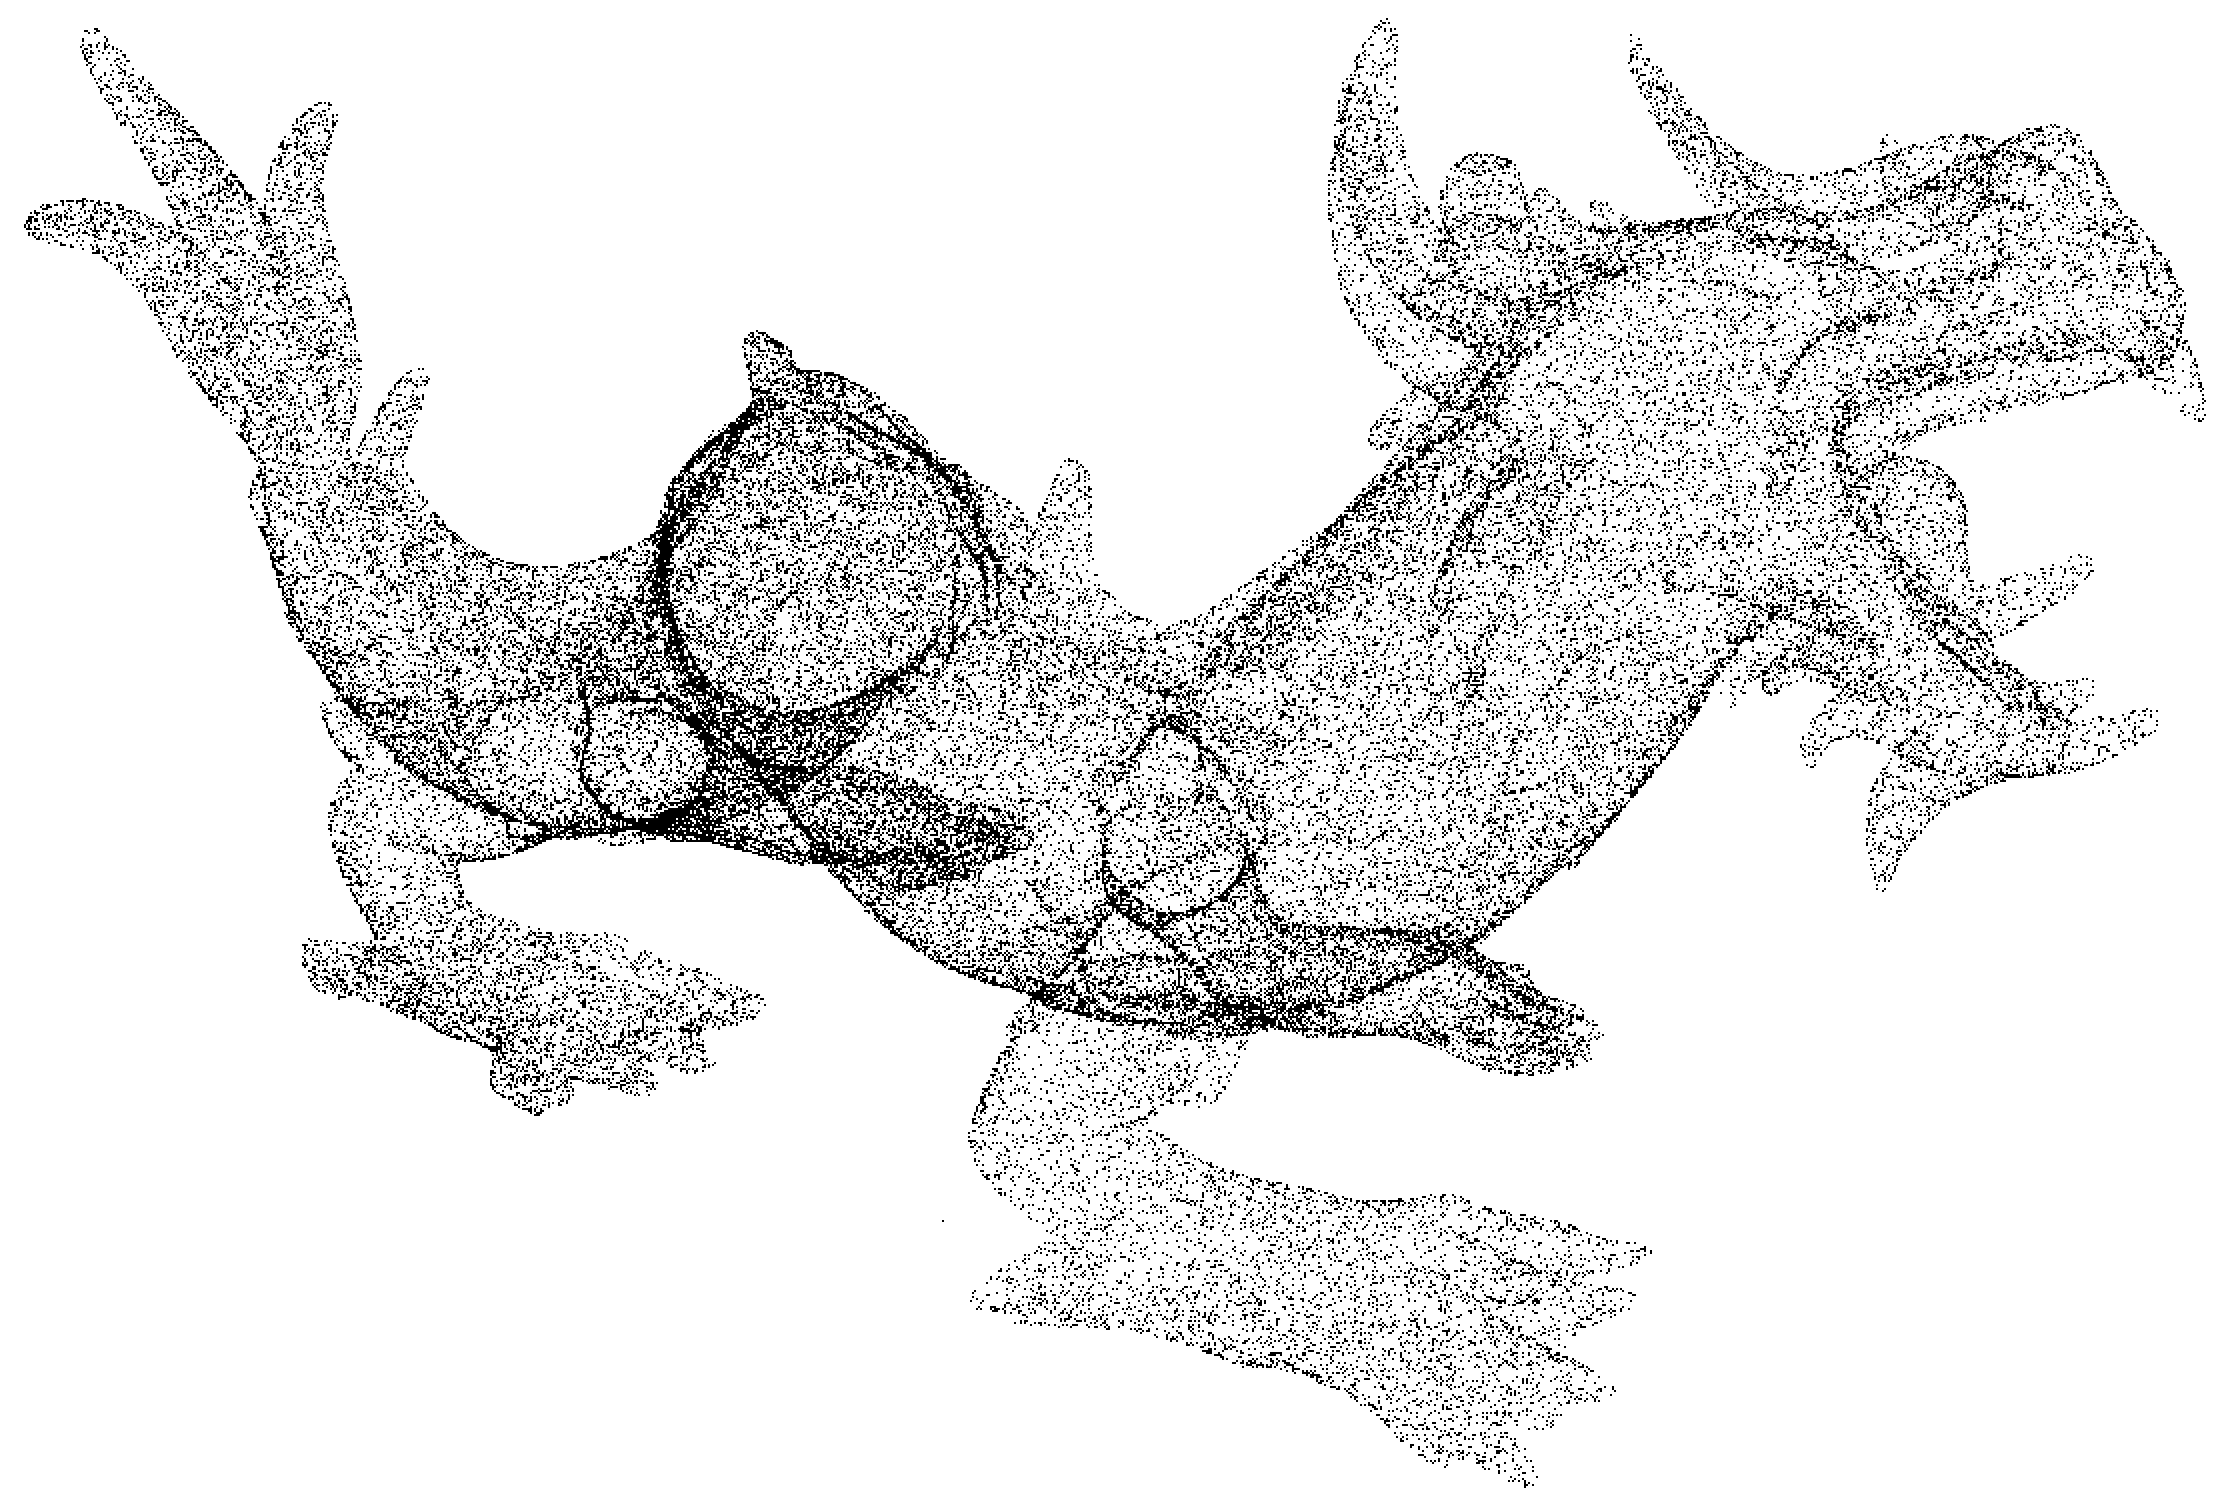
\includegraphics[width=.9\textwidth]{dragon_screenshot.png} \\
	\footnotesize{Modèle de Stanford Computer Graphics Laboratory}
\end{frame}

\begin{frame}
\frametitle{Scans bruts $\rightarrow$ modèle final}
	\begin{columns}
	\begin{column}[T]{.7\textwidth}
		\begin{itemize}
		\item Planification des scans / photos
			\\ p.ex. ajouter marqueurs visuels
		\item Filtrage bruit, outliers
		\item Recalage:
			\begin{itemize}
				\item Mettre plusieurs scans dans même repère
				\item Transformation rigide \\
					translation, rotation, (redimensionnement)
				\item Multiplication matricielle en coordonnées homogènes
				\item Recalage brut (semi-automatisé)
					\\ identifier correspondances, comparer formes, ...
				\item Recalage précis: ICP
			\end{itemize}
		\item Combinaison photo + nuage $\rightarrow$ colorisation
		\item Maillage, feature detection, CAD, ...
		\end{itemize}
	\end{column}
	\begin{column}[T]{.3\textwidth}
		{\footnotesize Marqueurs: \cite{Lerm2009}} \\
		\includegraphics[width=\textwidth]{markers.png}
		\vspace{1cm}
		{\footnotesize Colorisation: \cite{Lich2011} } \\
		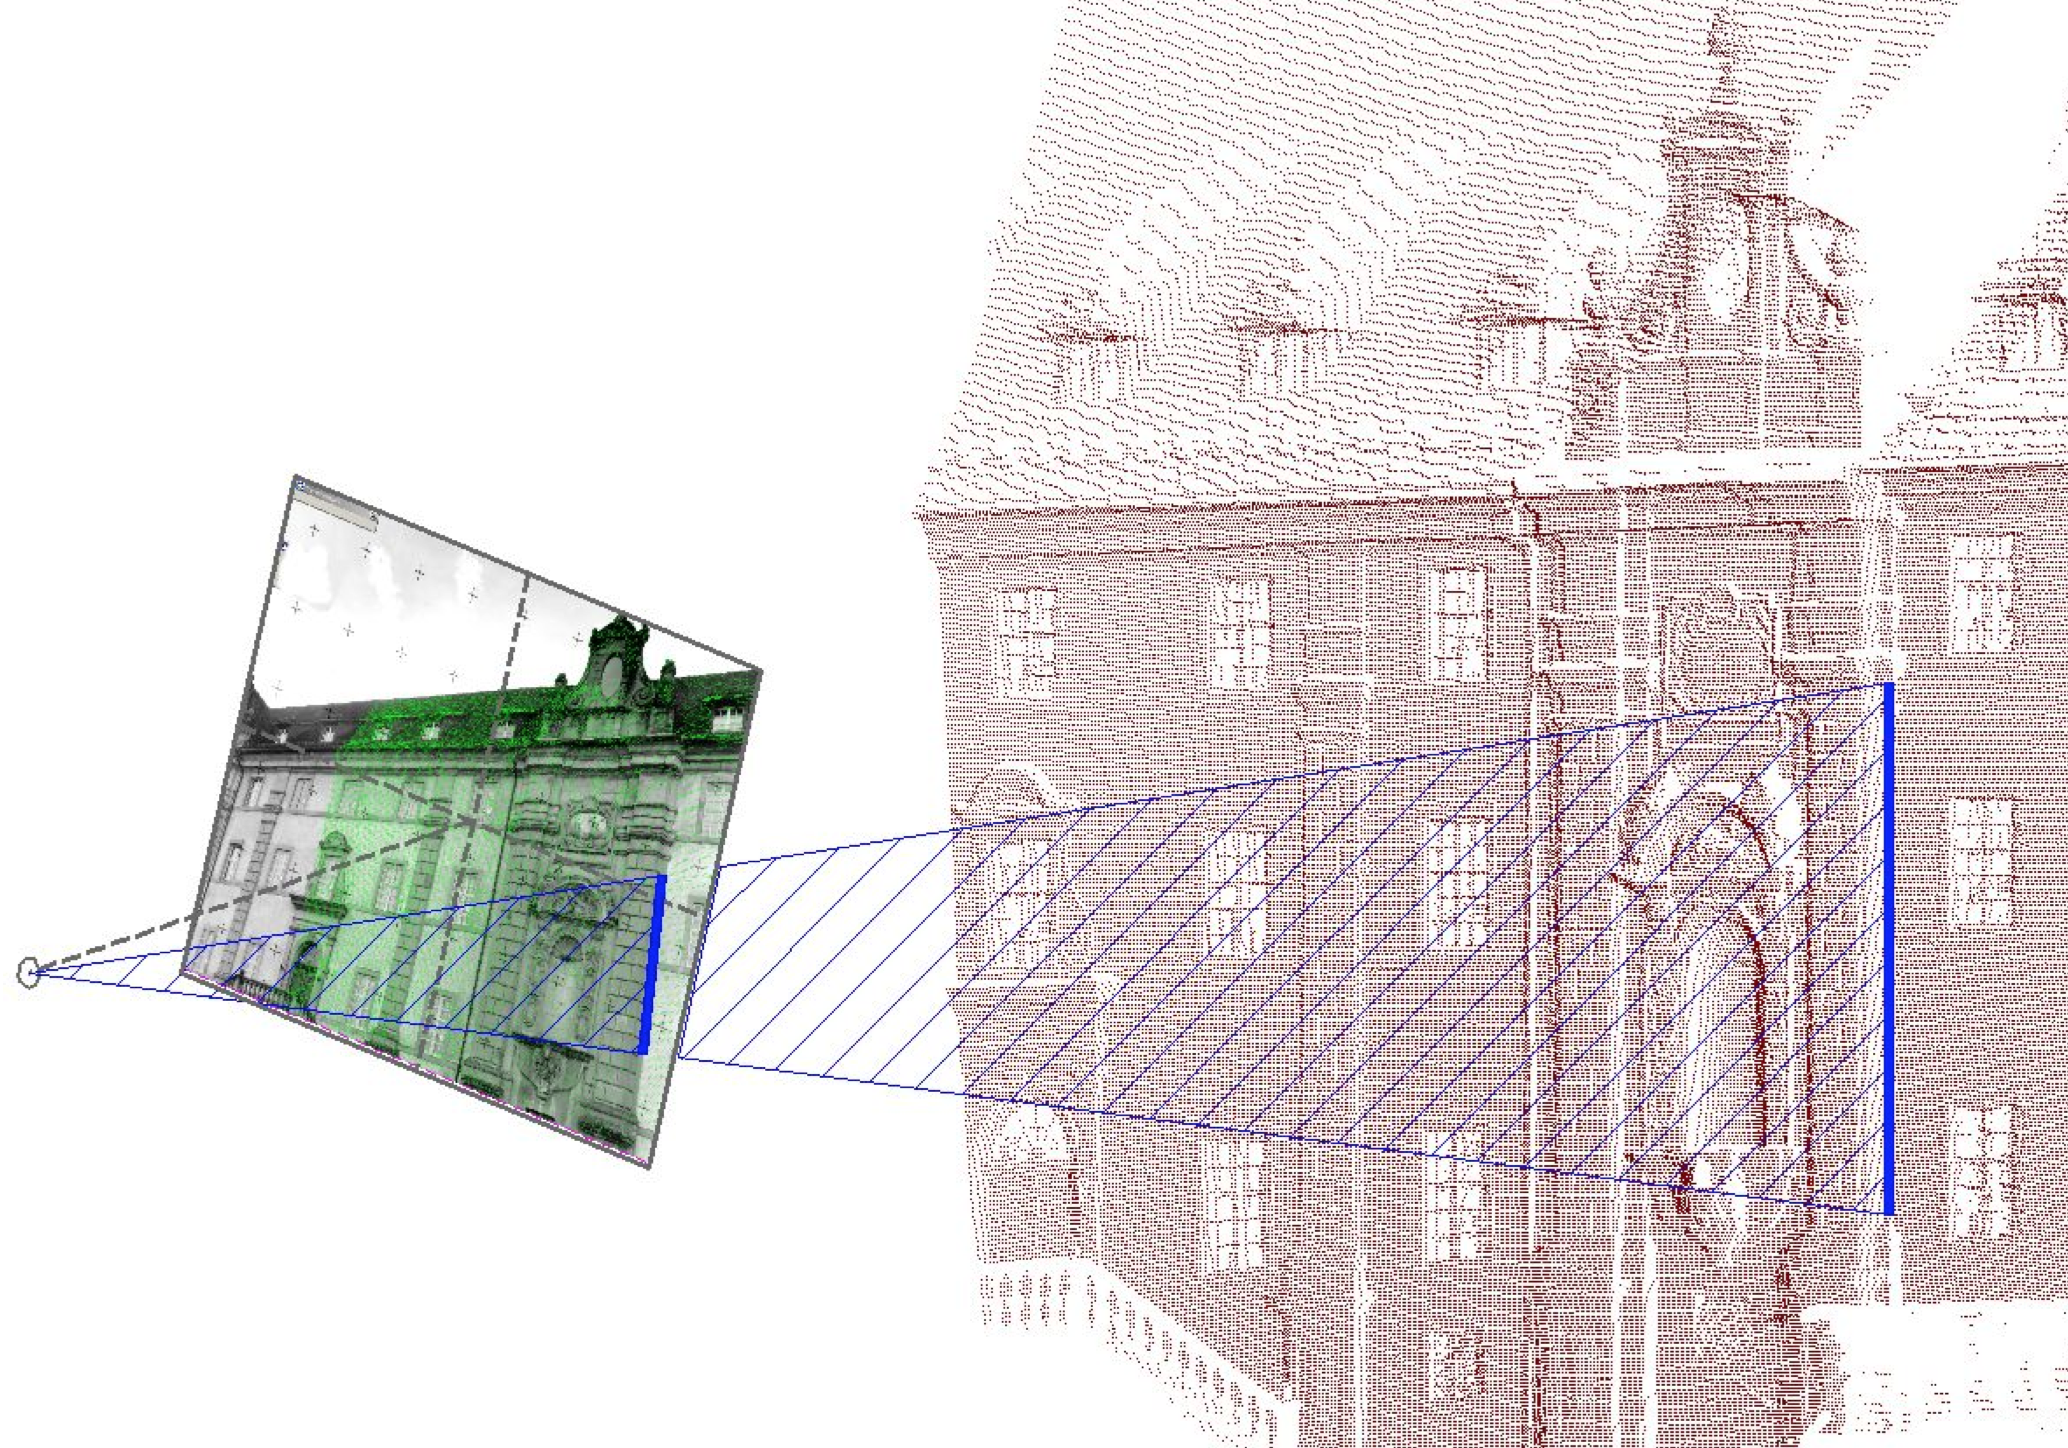
\includegraphics[width=\textwidth]{imagetocloud.png}
	\end{column}
	\end{columns}
\end{frame}

\begin{frame}
\frametitle{Recalage - Exemple 1}
	\center Recalage de 4 scans \footnotesize{\cite{Maka2006}}
	\vspace{5mm}
	\begin{columns}
	\begin{column}[T]{.5\textwidth}
		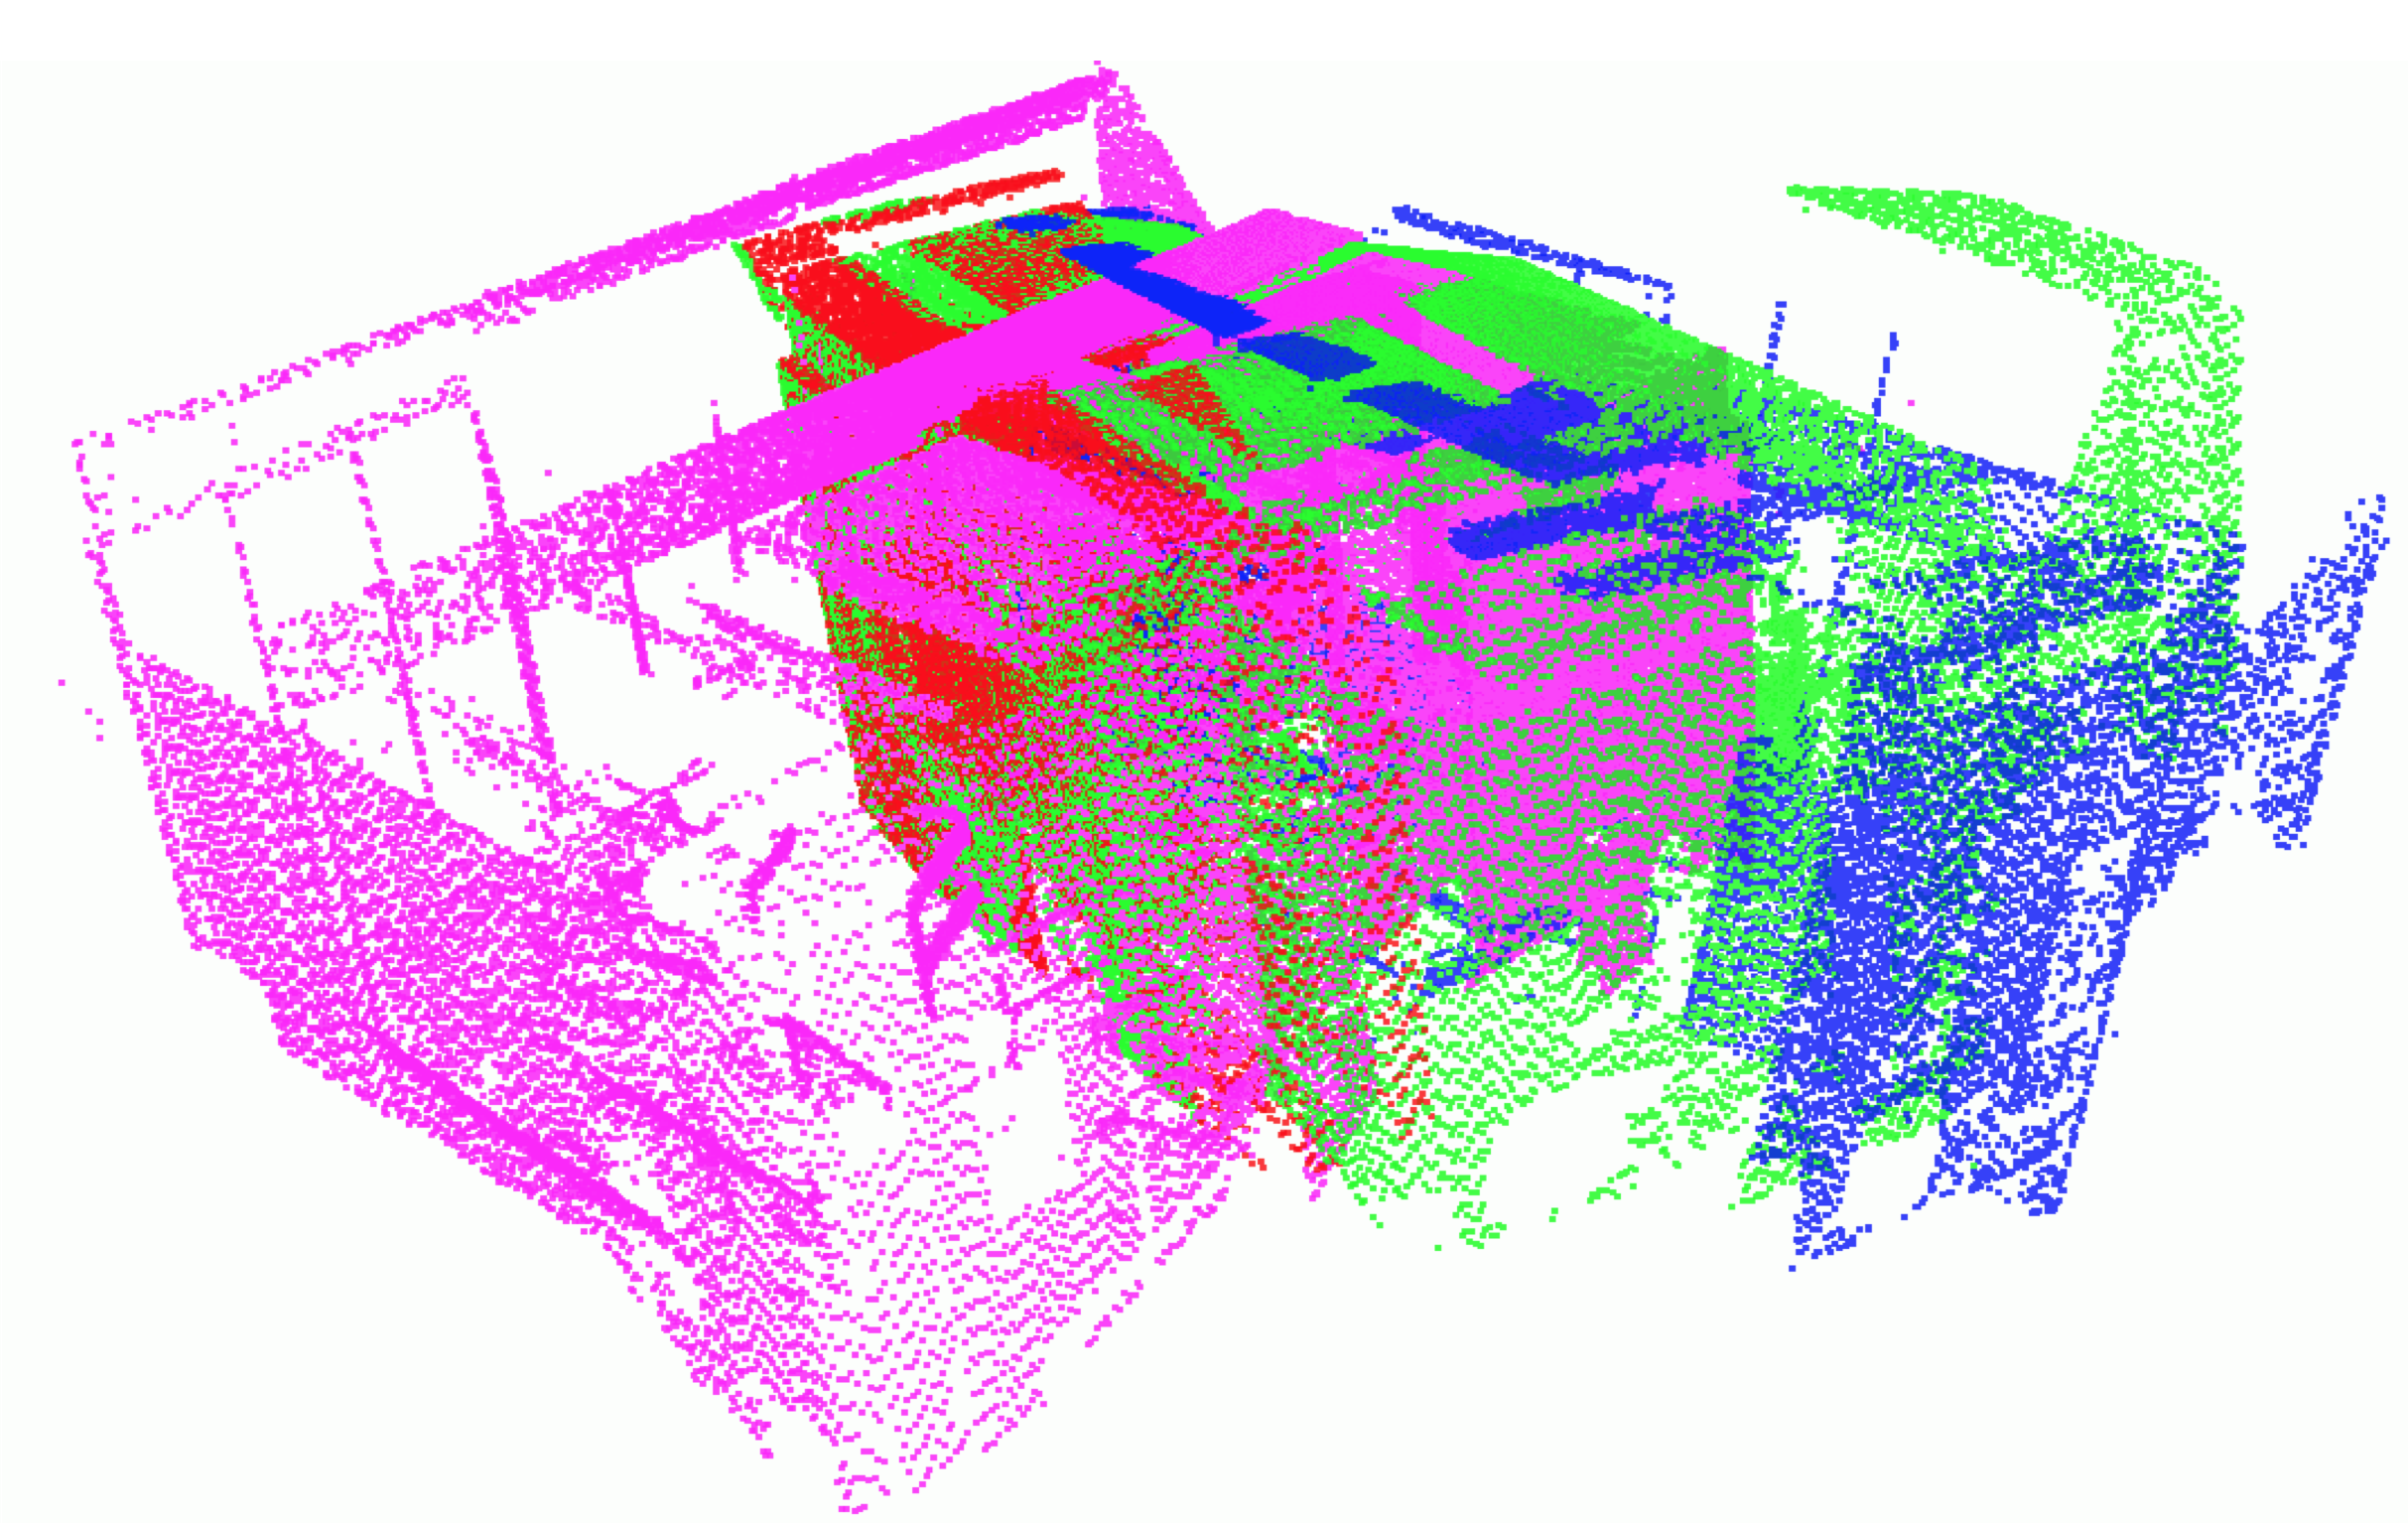
\includegraphics[height=4cm]{pre_reg.png}
		\center \Large{Avant}
	\end{column}
	\begin{column}[T]{.5\textwidth}
		\includegraphics[height=4cm]{post_reg.png}
		\center \Large{Après}
	\end{column}
	\end{columns}
\end{frame}

\begin{frame}
\frametitle{Recalage - Exemple 2}
	\center Recalage de 2 scans { \footnotesize \cite{Mati2011} }
		\\ avec overlap partiel
	\vspace{5mm}
	\begin{columns}
	\begin{column}[T]{.6\textwidth}
		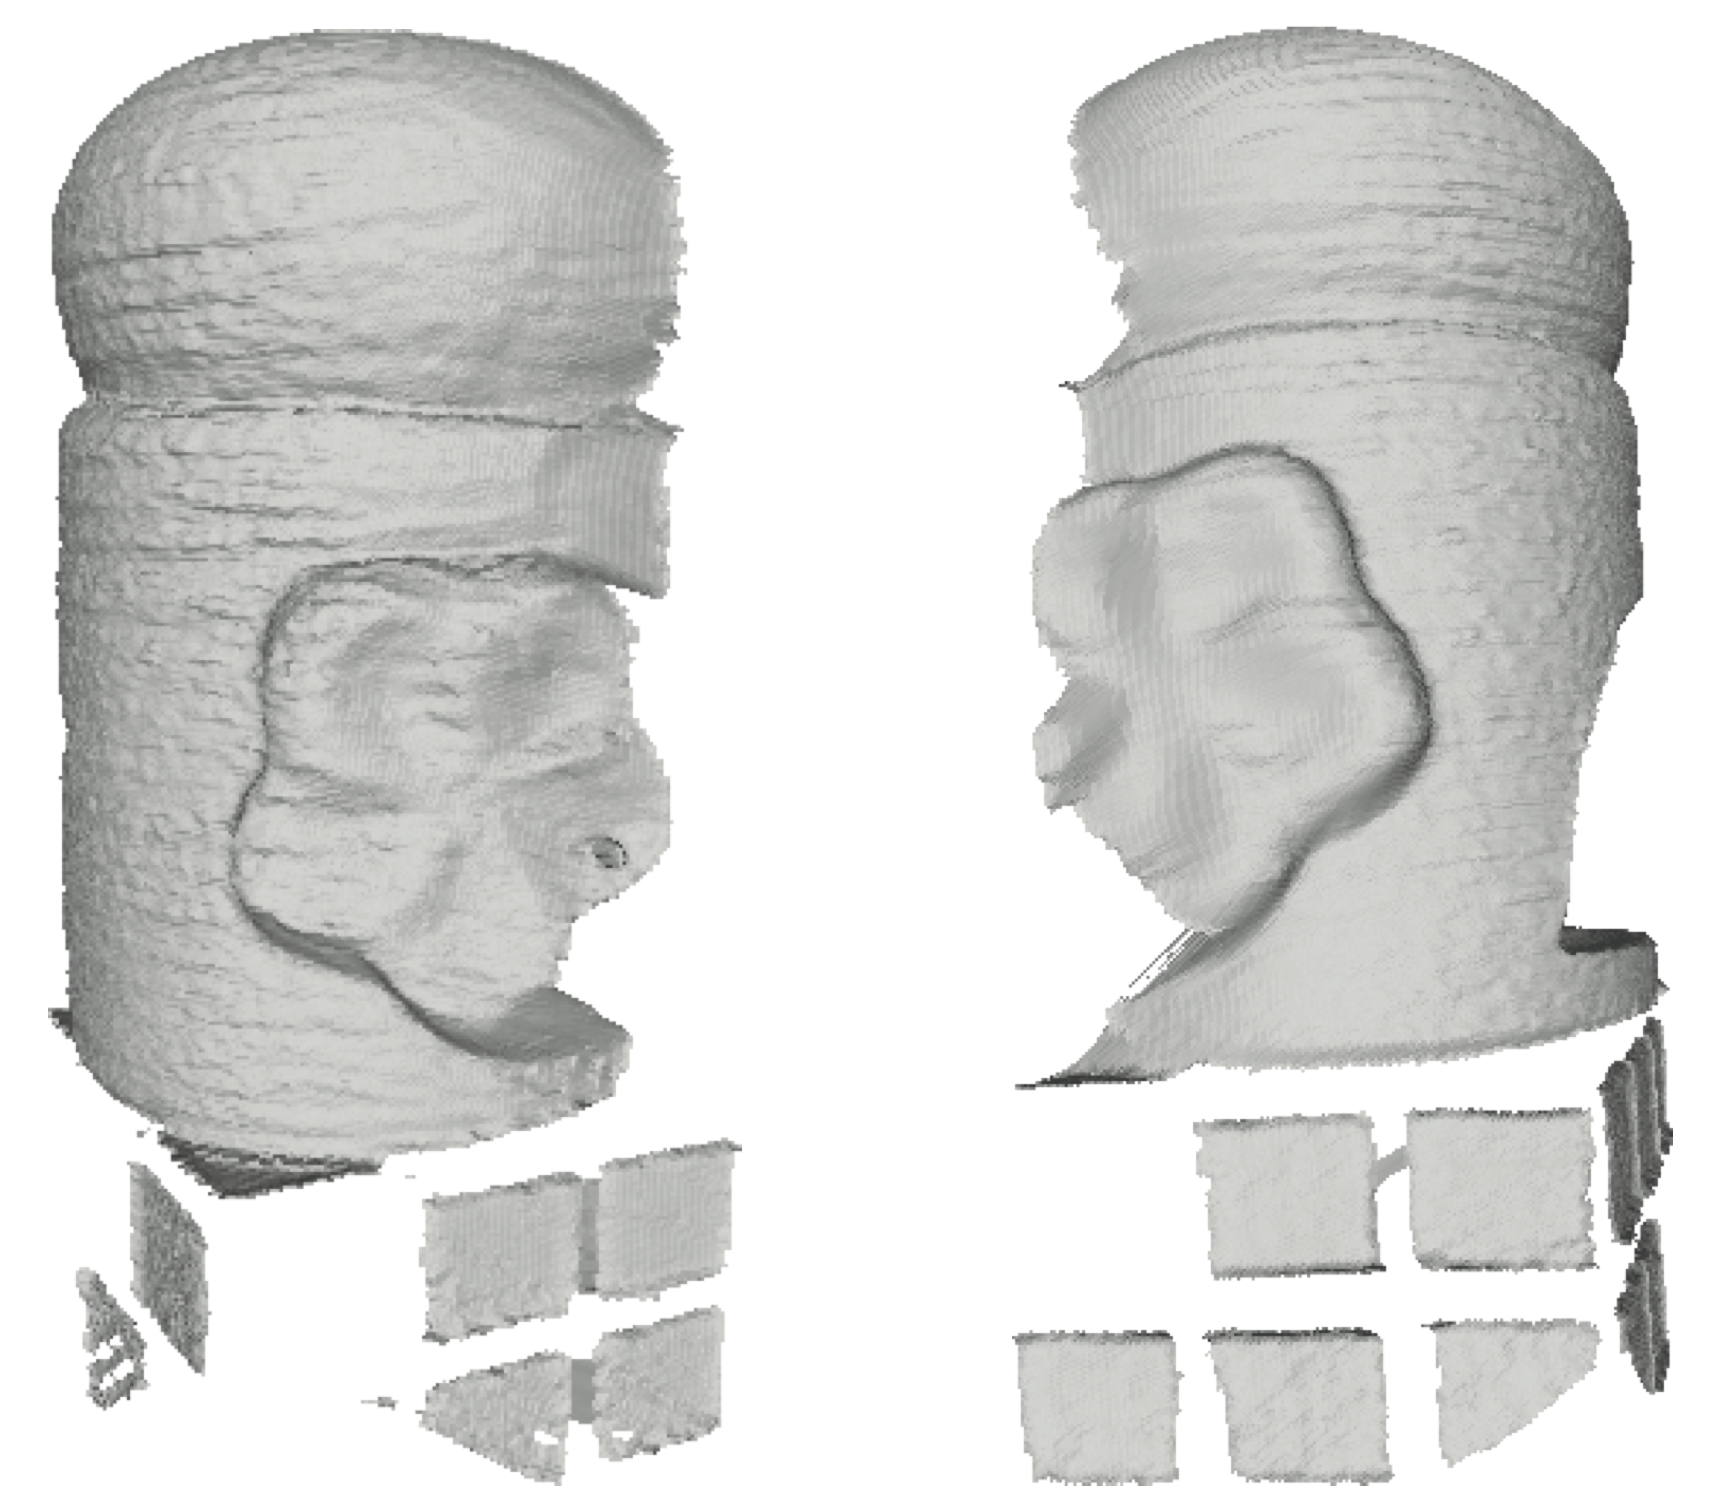
\includegraphics[height=5cm]{pre_reg2.png}
		\center \Large{Avant}
	\end{column}
	\begin{column}[T]{.3\textwidth}
		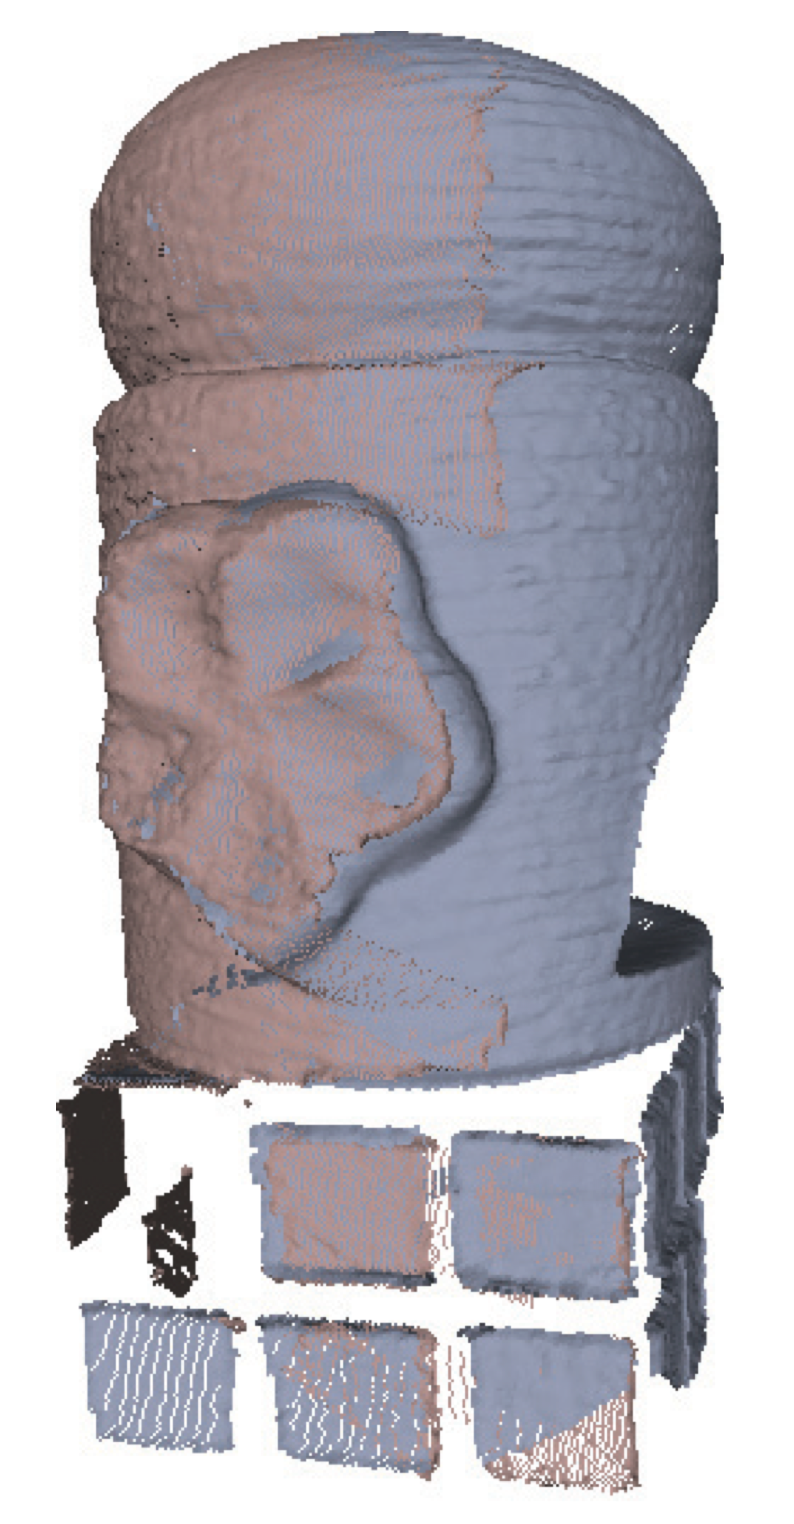
\includegraphics[height=5cm]{post_reg2.png}
		\center \Large{Après}
	\end{column}
	\end{columns}
\end{frame}

\begin{frame}
\frametitle{Projet de mémoire}
	\begin{itemize}
	\item Recalage et fusion
		\\ scans à grande distance + scans de détails
	\item Densité faible du modèle complet
	\item Grands nombres de points $\rightarrow$ algorithmes efficaces
	\item Développer méthode/algorithmes, établir workflow nécessaire
		\\ i.e. types de scans, photos requis
	\item Projets de documentation 3D (LISA ULB)
		\begin{itemize}
		\item Hôtel de Ville de Bruxelles
		\item Grotte avec gravures préhistoriques
		\end{itemize}
	\end{itemize}
	\begin{columns}
		\begin{column}[T]{.5\textwidth}
			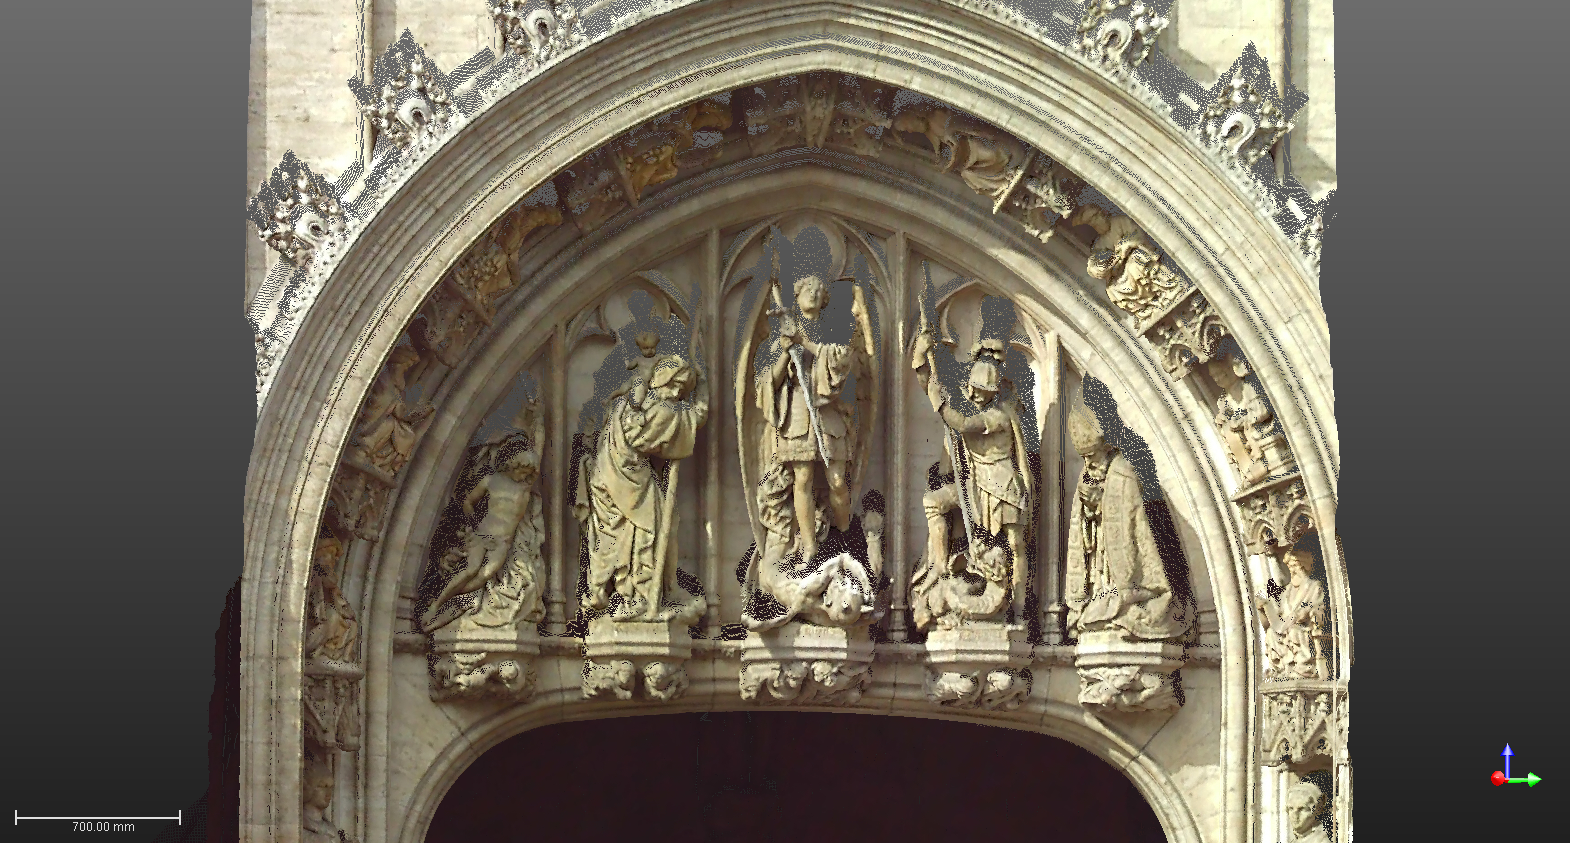
\includegraphics[width=\textwidth]{HotelDeVille_08.png}
		\end{column}
		\begin{column}[T]{.5\textwidth}
			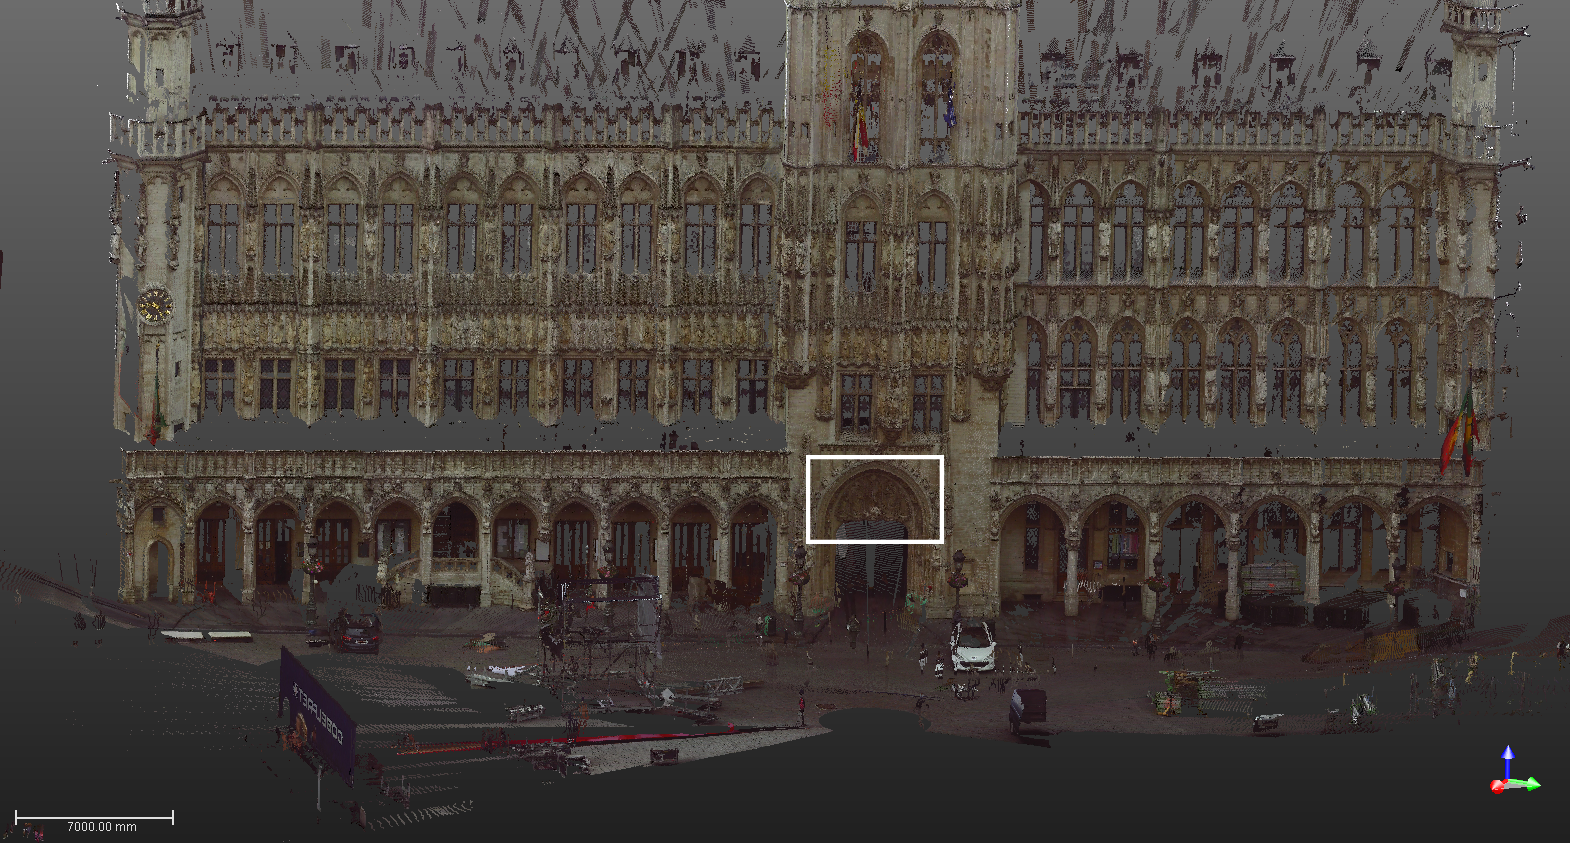
\includegraphics[width=\textwidth]{HotelDeVille_06rect.png}
		\end{column}
	\end{columns}
\end{frame}

\begin{frame}
\frametitle{Quelques techniques/algorithmes}
	\begin{block}{Nuages de points}
		\begin{description}[Recalage par photos]
		\item[ICP] Recalage précis, minimisation distances
		\item[Generalized-ICP] Approximation de surface par distribution des points
		\item[4PCS] Correspondance de 4-points congruents
		\item[Keypoints] Identifier points marquants
		\item[Recalage par photos] Correspondances sur photos associés aux nuages
		\end{description}	
	\end{block}
	
	\begin{block}{Photogrammétrie}
		\begin{description}[Appariement dense]
		\item[Reconstruction] Trouver position 3D à partir de photos
		\item[Appariement dense] Photos $\rightarrow$ carte de profondeur
		\item[Zônes d'intérêt] Points communs sur les photos
		\item[Hough Transform] Identifier droites
		\end{description}
	\end{block}
\end{frame}

\begin{frame}
\frametitle{Iterative Closest Point {\footnotesize \cite{Besl1992}}}
	\begin{itemize}
	\item 2 nuages de points déjà recalés approximativement
	\item \textbf{Cible} reste fixe, \textbf{Source} est transformée \\
		\begin{enumerate}
		\item Former couples $(s_i, c_i)$ de points +/- correspondants
			\\ p.ex. points les plus proches
		\item Métrique d'erreur, p.ex $\sum_i \| s_i - c_i \|^2$
		\item Transformer \textf{source} pour minimiser erreur
			\\ méthodes fermées, p.ex. rotation en quaternion
		\item Répéter jusqu'à erreur $<$ seuil
		\end{enumerate}
	\item Plusieurs variantes {\footnotesize \cite{Rusi2001}}
	\item \emph{Point-to-plane}: Plans tangents de \textbf{cible}
	\item \emph{Generalized-ICP}: Points $=$ variables aléatoires {\footnotesize \cite{Sega2009}}
	\end{itemize}
\end{frame}

\begin{frame}
\frametitle{4-Points Congruent Sets {\footnotesize \cite{Aige2008}}}
	\begin{itemize}
	\item {4-Points} $=$ ensemble de 4 points coplanaires. Procédure:
		\begin{enumerate}
		\item Choisir alétoirement \emph{4-Points} \textbf{base} dans \textbf{cible}
		\item Trouver plusieurs \emph{4-Points} congruents à \textbf{base} dans \textbf{source}
			\\ $=$ liées par transformation rigide
		\item Chercher celui qui donne le meilleure recalage
		\item Répéter (RANSAC)
		\end{enumerate}
	\item Pas besoin de recalage initial
	\item Résistant au bruit (outliers)
	\item \emph{K-4PCS}: Utilise des keypoints $\rightarrow$ Peut avoir densités différentes {\footnotesize \cite{Thei2013}}
	\end{itemize}
	\center 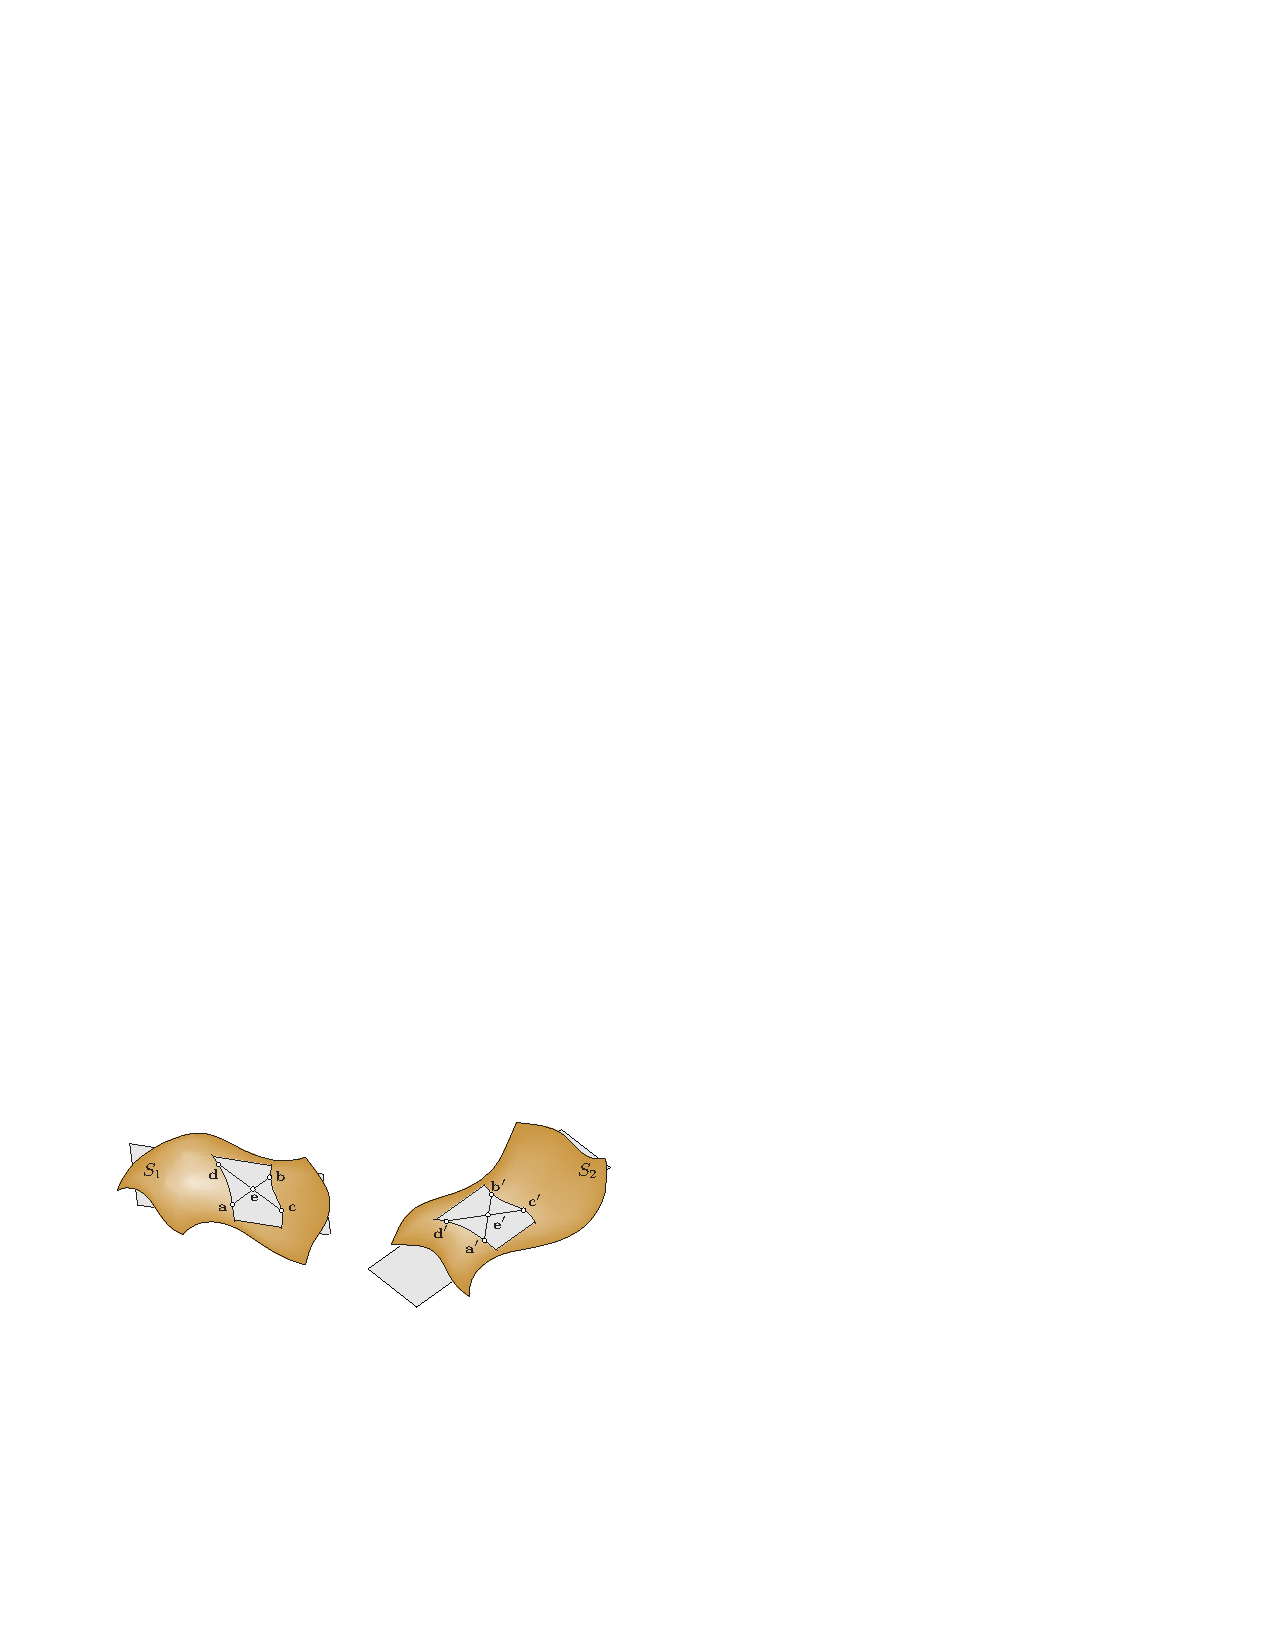
\includegraphics[width=.7\textwidth]{4pcs.pdf} {\footnotesize \cite{Aige2008}}
\end{frame}

\bibliographystyle{plain}
\footnotesize \bibliography{../references}

\end{document}
